\input{../../main.tex}

\setphysstyle{ГЦФО 8}{Вступительная олимпиада}{06.09.2016}

\begin{document}

\Large

\task{ Первую половину пути Баба-Яга летела со скоростью 20
  км/ч. Затем видимость ухудшилась, и половину оставшегося времени
  она пролетела со скоростью 10 км/ч. В этот момент у неё сломалась
  метла, и ей, чтобы успеть на встречу с Лешим, пришлось оставшееся
  время идти пешком со скоростью 5 км/ч. Найти среднюю скорость
  Бабы-Яги.}

\taskpic{ Для облегчения подъёма грузов часто применяют ворот,
  состоящий из двух валов, неподвижно закреплённых на одной оси. При
  работе такого ворота трос, сматываясь с одного вала, одновременно
  наматывается на другой. Какую силу $F$ нужно приложить к рукоятке
  ворота длиной $l$, чтобы груз массы $m$ находился в равновесии?
  Весом блока и трением пренебречь. Радиус малого вала $r$, большого
  --- $R$. }  {
  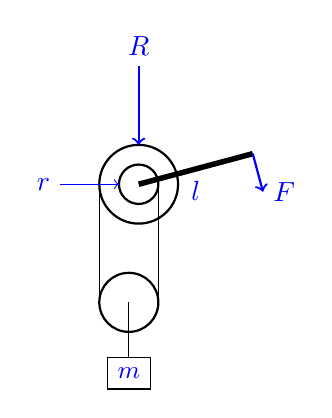
\begin{tikzpicture}
    \draw[thick] (2,3.5) circle (0.25);
    \draw[thick] (2,3.5) circle (0.5);
    \draw (2.25,3.5) -- (2.25,2);
    \draw (1.5,3.5) -- (1.5,2);
    \draw[thick] (1.875,2) circle (0.375);
    \draw (1.875,2) -- (1.875,1.3);
    \draw (1.6,1.3) rectangle (2.15,0.9) node[midway,blue]
    {\small $m$};
    \draw[line width=0.07cm] (2,3.5) -- ++(15:1.5cm)
    node[midway,below,blue] {$l$};
    \draw[thick,blue,->] (2,3.5) ++ (15:1.5cm) -- ++(-75:0.5cm)
    node[right,blue] {$F$};
    \draw[thick,blue,->] (2,3.5) ++(90:1.5cm) node[above] {$R$} --
    ++(270:1cm);
    \draw[blue,->] (1,3.5) node[left] {$r$} -- (1.75,3.5);
  \end{tikzpicture}
}
% Лукашик, 14.24

\taskpic{ Сплошной шарик подвешен в сосуде на двух одинаковых лёгких
  нитях, как показано на рисунке. Свободные концы нитей закреплены на
  одной высоте. После того как сосуд заполнили водой, и шарик оказался
  полностью погруженным в воду, натяжение нитей не изменилось.
  Определите плотность $\rho$ материала, из которого изготовлен
  шарик. Плотность воды $\rho_0 = 1000\mbox{ кг/м}^3$.}
{
  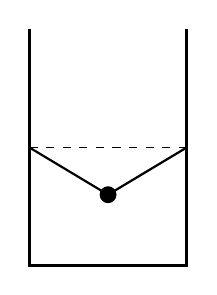
\begin{tikzpicture}
    \draw[very thick] (0,3) -- (0,0) -- (2,0) -- (2,3);
    \draw[dashed] (0,1.5) -- (2,1.5);
    \draw[thick] (0,1.5) -- (1,.9) -- (2,1.5);
    \draw[fill=black] (1,.9) circle (0.1cm);
  \end{tikzpicture}
}
% Московская городская олимпиада, 2007

\end{document}


%%% Local Variables: 
%%% mode: latex
%%% TeX-engine:xetex
%%% TeX-PDF-mode: t
%%% End:
